% ----------------------------------------------------------------------
%  Pracovní úkoly
% ----------------------------------------------------------------------
\section{Pracovní úkoly}

\begin{enumerate}
\item Změřte modul pružnosti v tahu E oceli z protažení drátu.

\item Změřte modul pružnosti v tahu E oceli a mosazi z průhybu trámku.

\item Výsledky měření graficky znázorněte, modul pružnosti určete pomocí lineární regrese.

\end{enumerate}

% ----------------------------------------------------------------------
%  Teoretická část
% ----------------------------------------------------------------------
\section{Teoretická část}

\subsection{Protažení drátu}

Pro měření modulu pružnosti \(E\) využijeme Hookův zákon

\begin{equation}
    \sigma = E \cdot \epsilon
\end{equation}

kde \(\sigma\) je normálové napětí a \(\epsilon\) relativní prodloužení. Tento zákon platí pouze v oblasti pružné deformace, proto budeme měření provádět i zpětně, abychom ověřili, že je deformace vratná a my jsme tak nepřekročili mez pružnosti. Na obrázku \ref{fig:aparatura-protazeni-dratu} je znázorněno schéma aparatury této metody.

\begin{figure}[h]
    \centering
    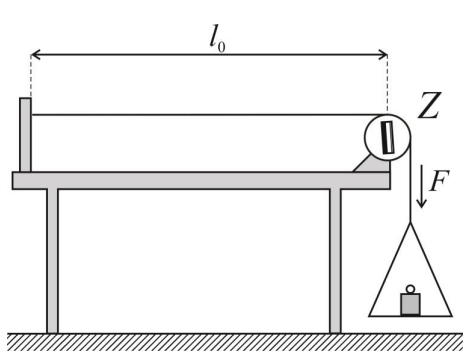
\includegraphics[width=0.5\linewidth]{09 - Měření modulu pružnosti v tahu//Protokol_modul pružnosti//img/Aparatura_protažení drátu.png}
    \caption{Aparatura měření protažení drátu}
    \label{fig:aparatura-protazeni-dratu}
\end{figure}

Působíme silou \(F\) na drát délky \(l_0\) o průřezu \(S\) pomocí závaží zavěšených na jeden konec drátu. Na druhém konci je drát pevně upevněn. Potom pro prodloužení drátu \(\Delta l\) platí

\begin{equation}
    \Delta l = \frac{1}{E} \frac{l_0 F}{S}
\end{equation}

Napětí \(\sigma\) lze vyjádřit jako

\begin{equation}
    \sigma = \frac{F}{S}
\end{equation}

a relativní prodloužení \(\epsilon\) jako

\begin{equation}
    \epsilon = \frac{\Delta l}{l_0}
\end{equation}

Odtud můžeme modul pružnosti \(E\) spočítat jako

\begin{equation}
    E = \frac{l_0 F}{\Delta l \cdot S}
\end{equation}

Pro určení délky prodloužení drátu využijeme zrcátka, které je upevněno na kladce přes kterou je veden drát. Dalekohledem pozorujeme odrazem od zrcátka stupnici. V závislosti na otočení zrcátka odečteme počet dílků na stupnici, o které se zrcátko pootočilo.

\newpage

Úhel pootočení zrcátka \(\Delta \alpha\) udává prodloužení drátu jako

\begin{equation}
    \Delta l = r \cdot \Delta \alpha
\end{equation}

kde r je poloměr kladky.

Pro výpočet úhlu \(\Delta \alpha\) z rozdílu délek stupnice před a po zatížení \(n - n_0\) využijeme

\begin{equation}
    tg (2 \Delta \alpha) = \frac{n - n_0}{L}
\end{equation}

kde \(L\) je vzdálenost dalekohledu od zrcátka.

Protože se pohybujeme nízkých hodnotách úhlu \(\Delta \alpha\) můžeme aproximovat \(tg(\alpha) \approx \alpha\) a dostáváme tedy

\begin{equation}
    \Delta \alpha \approx \frac{n - n_0}{2L}
\end{equation}

\subsection{Průhyb trámku}

Ve druhé metodě využijeme prohnutí trámku upevněného břity na jeho koncích, který je uprostřed své délky zatížen. Toto schéma popisuje obrázek \ref{fig:aparatura-prohnuti-tramku}. Vzdálenost mezi břity označme \(l\) a výšku a šířku trámku s obdélníkovým kolmým průřezem jako výšku \(b\) a šířku \(a\).

\begin{figure}[h]
    \centering
    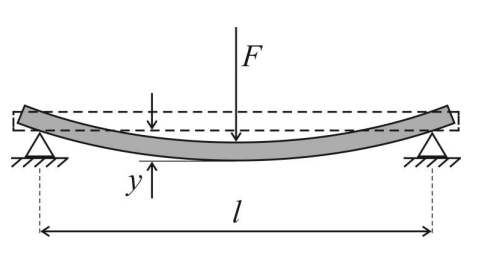
\includegraphics[width=0.5\linewidth]{09 - Měření modulu pružnosti v tahu//Protokol_modul pružnosti//img/Aparatura_průhyb trámku.png}
    \caption{Aparatura měření prohnutí trámku}
    \label{fig:aparatura-prohnuti-tramku}
\end{figure}

Pro velikost průhybu \(y\), který vznikne působením síly F ve středu, platí

\begin{equation}
    y = \frac{F l^3}{48 E I_p}
\end{equation}

kde \(I_p\) se nazývá plošný moment setrvačnosti průřezové plochy tyče vzhledem k vodorovné ose.

Odvozením z předchozí rovnice pro výpočet modulu pružnosti použijeme

\begin{equation}
    E = \frac{F l^3}{4 y a b^3}
\end{equation}


% ----------------------------------------------------------------------
%  Výsledky a zpracování měření
% ----------------------------------------------------------------------
\section{Výsledky a zpracování měření}

\subsection{Laboratorní podmínky}

    Měření bylo prováděno za laboratorních podmínek uvedených v tabulce \ref{tab:lab_pod}.

    \begin{table}[h]
        \centering
        \begin{tabular}{|c|c|c|} 
        \hline
            t / °C & p / hPa & vlhkost / \%RH  \\ 
        \hline
            23,6(4)   & 948,9(20)   & 40,6(25)            \\
        \hline
        \end{tabular}
        \caption{Laboratorní podmínky}
        \label{tab:lab_pod}
    \end{table}

\newpage

\subsection{Měření modulu E z protažení drátu}

V tabulce \ref{tab:vychozi-vzdalenosti} jsou uvedeny naměřené vzdálenosti jednotlivých částí aparatury. Nepřesnost měření délky \(l_0\) je nadhodnocena, než by ve skutečnosti přesnost svinovacího metru dovolovala, protože není přesně určeno místo, odkud kam se má drát měřit a navíc je obtížné přesné měření. Vzdálenost je tedy brána od konce upevnění drátu a na druhé straně je odhadnutý bod na kladce, kde působí maximální normálová síla na drát a nedochází zde k prokluzování drátu na kladce. Průměr kladky byl změřen posuvným měřidlem. Zde byl průměr měřen uprostřed kladky v místě, kudy prochází drát. K určení vzdálenosti \(L\) byl použit svinovací metr a k určení průměru drátu \(d\) mikrometr. Průměr drátu byl změřen třikrát v různých místech a s různě nakloněným mikrometrem, vždy byla ale změřena přesně stejná hodnota.

\begin{table}[h]
\centering
\begin{tabular}{|l|l|}
\hline
Délka drátu l_0 / m                 & 1,16(1)   \\ \hline
Průměr kladky 2r / m                 & 0,0383(1) \\ \hline
Vzdálenost stupnice od zrcátka L / m & 0,895(1)  \\ \hline
Průměr drátu d / m                   & 0,0005(01) \\ \hline
\end{tabular}
\caption{Naměřené výchozí vzdálenosti}
\label{tab:vychozi-vzdalenosti}
\end{table}

Odtud můžeme určit obsah kruhového průřezu drátu

\begin{equation}
    \nonumber
    S = 0,20(1) \; mm^2 = 2(01) \cdot 10^{-7} \; m^2
\end{equation}

V tabulce níže jsou uvedeny závislosti velikosti zatížení a protažení tyče. Působící síla je spočtena jako síla gravitační \(F = m \cdot g\), kde \(g = 9,81 m \cdot \; s^{-2}\) podle [2]. Hodnota \(n - n_0\) udává rozdíl dílků na stupnici z aktuálního a počátečního zatížení při 1 kg. Změna délky struny je odtud dopočtena podle (6) a (8). První tabulka odpovídá postupnému zatěžování a tabulka druhá zkracování struny.

\begin{table}[h]
\centering
\begin{tabular}{|c|c|c|c|}
\hline
Hmotnost závaží / kg & Síla / N & n - n\_0 / cm & Změna délky struny / cm \\ \hline
1                    & 9,8      & 0             & 0,0000                  \\ \hline
1,5                  & 14,7     & 1,3           & 0,0139(1)                  \\ \hline
1,6                  & 15,7     & 1,6           & 0,0171(1)                  \\ \hline
1,7                  & 16,7     & 1,8           & 0,0193(1)                  \\ \hline
1,8                  & 17,7     & 2,2           & 0,0235(1)                  \\ \hline
1,9                  & 18,6     & 2,4           & 0,0257(1)                  \\ \hline
2                    & 19,6     & 2,7           & 0,0289(2)                  \\ \hline
2,1                  & 20,6     & 2,9           & 0,0310(2)                  \\ \hline
2,2                  & 21,6     & 3,2           & 0,0342(2)                  \\ \hline
2,3                  & 22,6     & 3,5           & 0,0374(2)                  \\ \hline
2,4                  & 23,5     & 3,7           & 0,0396(2)                  \\ \hline
2,5                  & 24,5     & 4             & 0,0428(2)                  \\ \hline
2,6                  & 25,5     & 4,2           & 0,0449(2)                  \\ \hline
2,7                  & 26,5     & 4,5           & 0,0481(3)                  \\ \hline
2,8                  & 27,5     & 4,8           & 0,0514(3)                  \\ \hline
2,9                  & 28,4     & 5             & 0,0535(3)                  \\ \hline
\end{tabular}
\end{table}

\begin{table}[h]
\centering
\begin{tabular}{|c|c|c|c|}
\hline
Hmotnost závaží / kg & Síla / N & n - n\_0 / cm & Změna délky struny / cm \\ \hline
2,9                  & 28,4     & 5             & 0,0535(3)                  \\ \hline
2,8                  & 27,5     & 4,7           & 0,0503(3)                  \\ \hline
2,7                  & 26,5     & 4,5           & 0,0481(3)                  \\ \hline
2,6                  & 25,5     & 4,2           & 0,0449(2)                  \\ \hline
2,5                  & 24,5     & 3,9           & 0,0417(2)                  \\ \hline
2,4                  & 23,5     & 3,7           & 0,0396(2)                  \\ \hline
2,3                  & 22,6     & 3,4           & 0,0364(2)                  \\ \hline
2,2                  & 21,6     & 3,2           & 0,0342(2)                  \\ \hline
2,1                  & 20,6     & 2,9           & 0,0310(2)                  \\ \hline
2                    & 19,6     & 2,7           & 0,0289(2)                  \\ \hline
1,9                  & 18,6     & 2,4           & 0,0257(1)                  \\ \hline
1,8                  & 17,7     & 2,1           & 0,0225(1)                  \\ \hline
1,7                  & 16,7     & 1,9           & 0,0203(1)                  \\ \hline
1,6                  & 15,7     & 1,6           & 0,0171(1)                  \\ \hline
1,5                  & 14,7     & 1,3           & 0,0139(1)                  \\ \hline
1                    & 9,8      & 0             & 0                  \\ \hline
\end{tabular}
\end{table}

\newpage

Nepřesnost změny délky struny je dána podle metody přenosu chyb jako

\begin{equation}
    \sigma_\Delta_l = \Delta l \sqrt{\frac{\sigma^2_r}{r^2}+\frac{\sigma^2_L}{L^2}}
\end{equation}

Modul pružnosti spočítáme nejprve podle rovnice (5)

\begin{equation}
    \nonumber
    E = 84(4) GPa
\end{equation}

kde chyba je určena metodou přenosu chyb

\begin{equation}
    \sigma_E = E \sqrt{\frac{\sigma^2_l__0}{l^2_0}+\frac{\sigma^2_\Delta__l}{\Delta l^2}+\frac{\sigma^2_S}{S^2}}
\end{equation}

\begin{figure}[h]
    \centering
    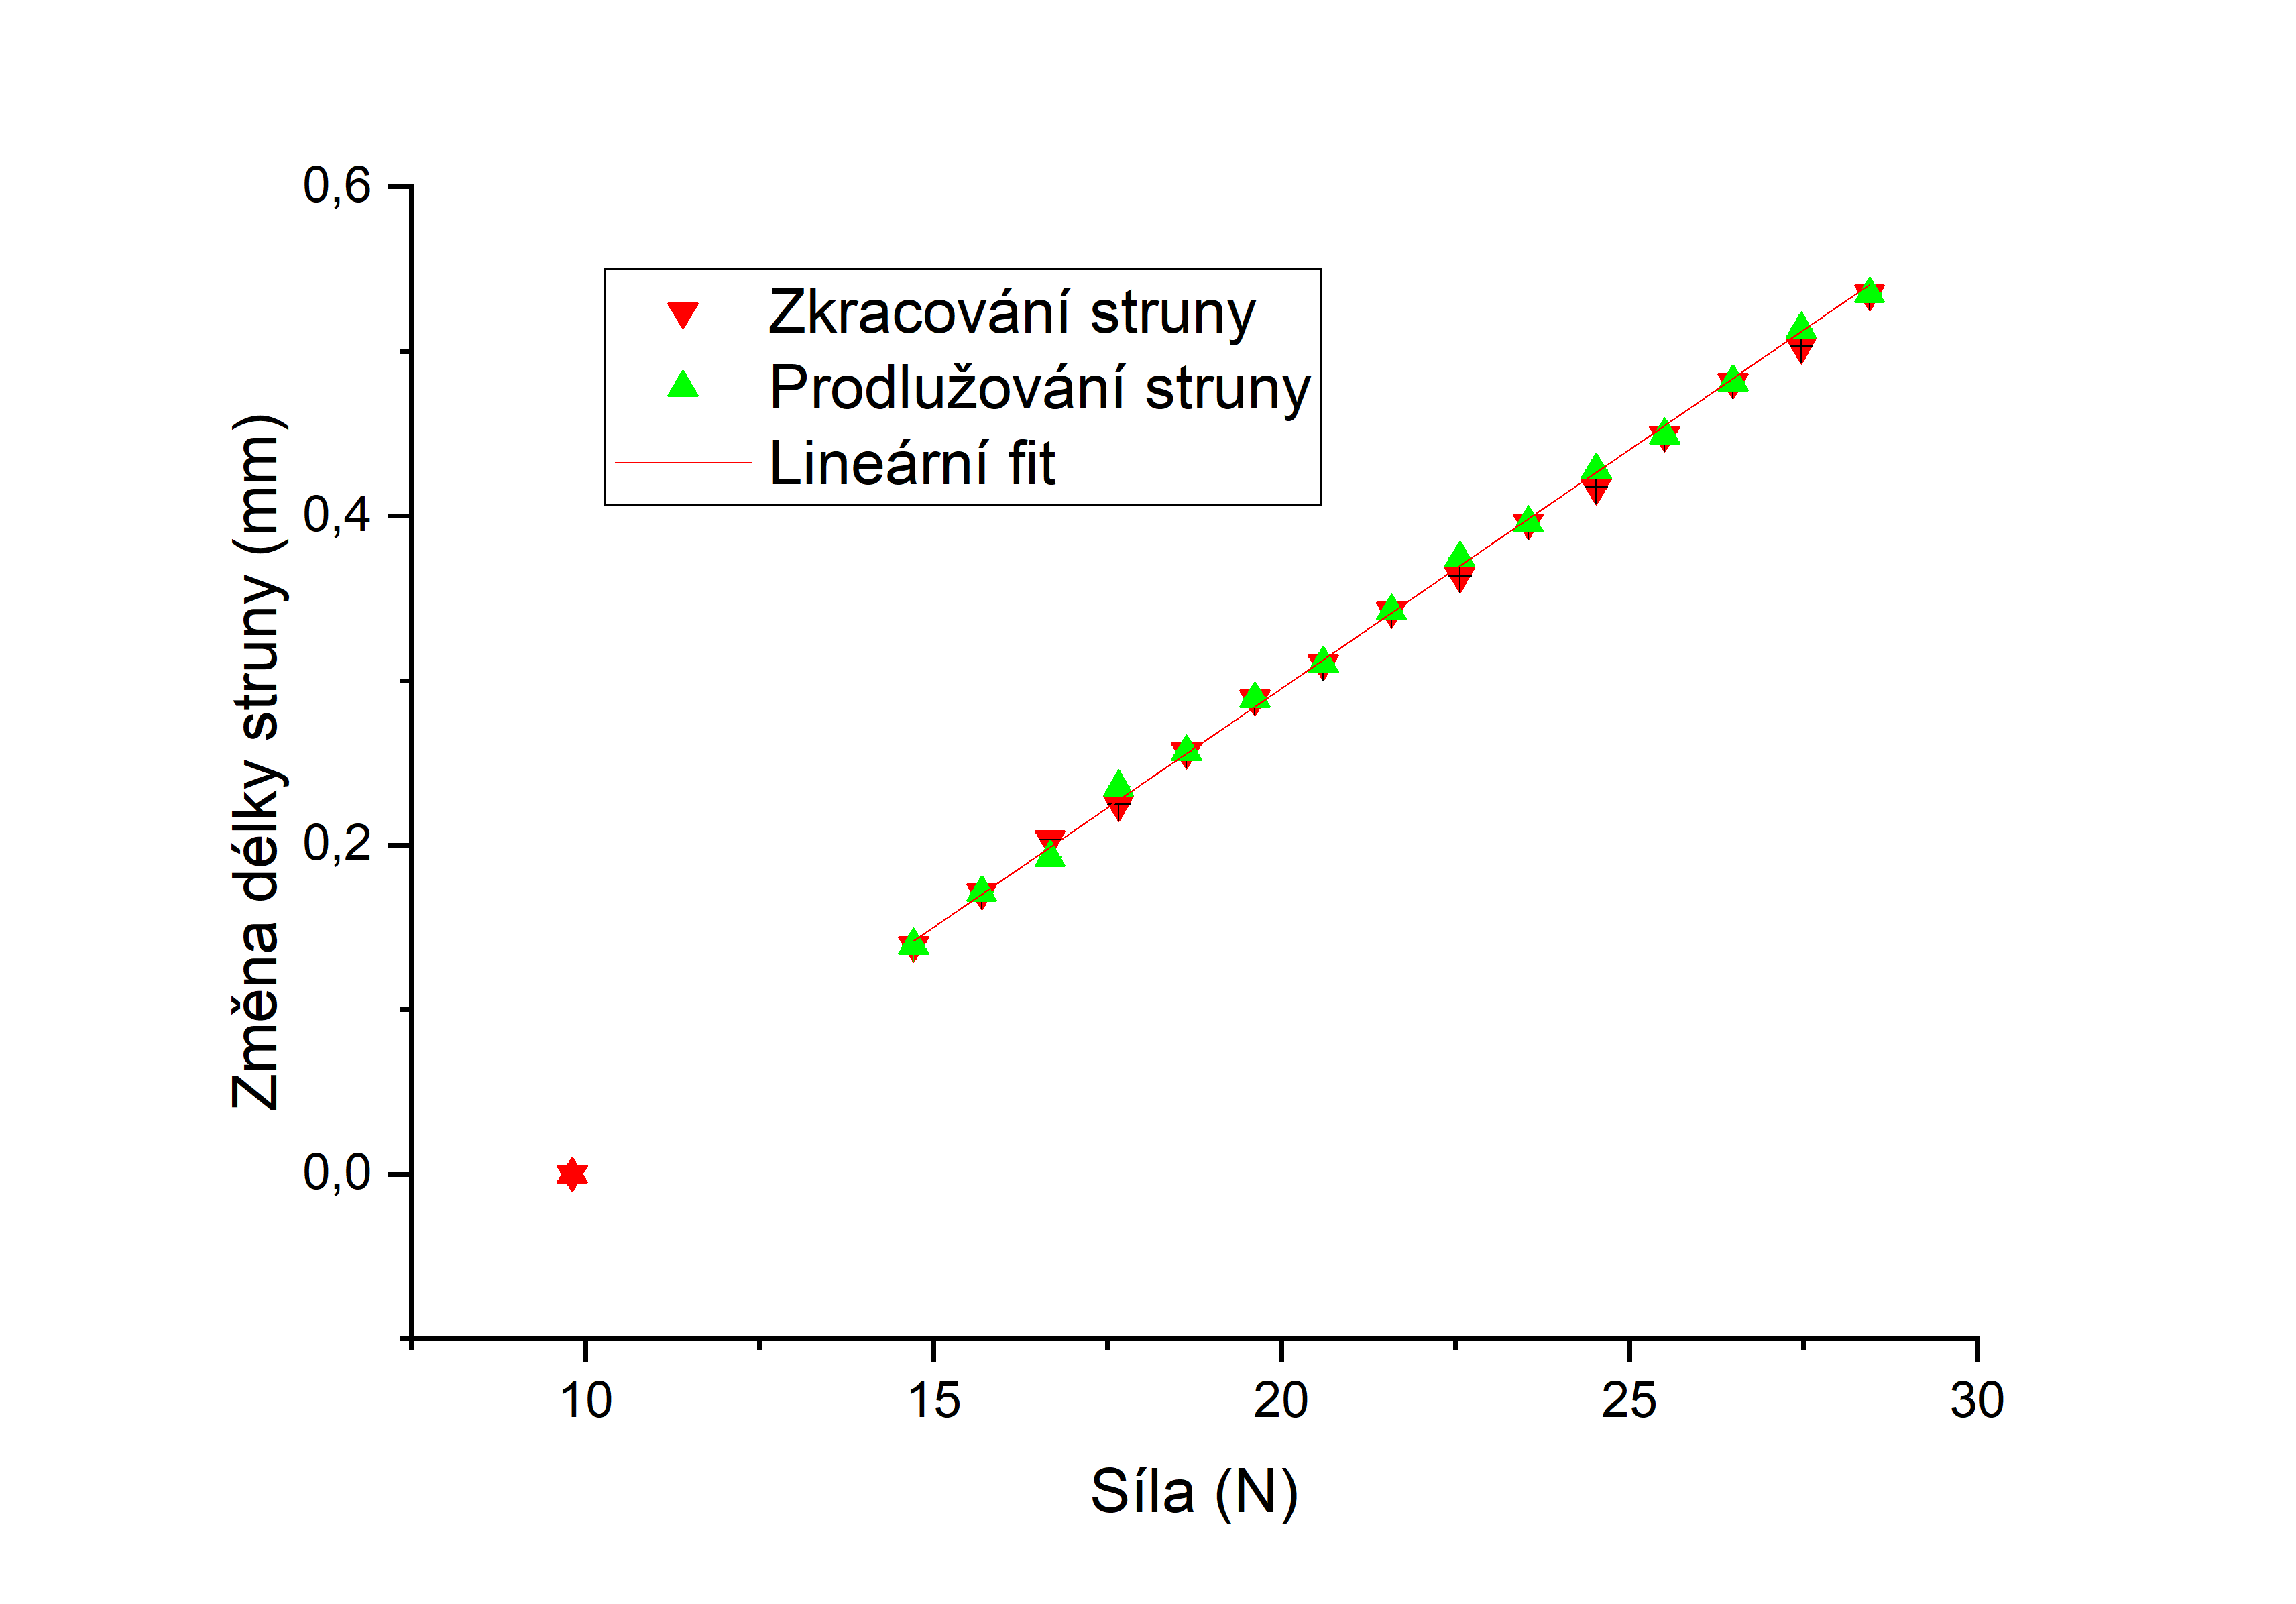
\includegraphics[width=0.85\linewidth]{09 - Měření modulu pružnosti v tahu//Protokol_modul pružnosti//img/Změna délky struny.png}
    \caption{Závislost změny délky struny na působící síle}
    \label{fig:delka-struny}
\end{figure}

% ----------------------------------------------------------------------
%  Diskuse výsledků
% ----------------------------------------------------------------------			
\section{Diskuse výsledků}

% ----------------------------------------------------------------------
%  Závěr
% ----------------------------------------------------------------------
\section{Závěr}
